%\documentclass[openright,twoside,headsepline]{scrbook}
%\usepackage[applemac]{inputenc}
%\usepackage{graphicx,xcolor,hyperref} % obsolete in HU-diss
%\usepackage[round,authoryear]{natbib}
%\setlength\bibhang{2em} 
%
%
%\KOMAoptions{numbers=noenddot}
\usepackage{amsmath,amssymb,amsfonts,amsthm,epigraph,scrpage2}
\usepackage[ngerman,english]{babel}
\definecolor{Cayenne}{rgb}{0.502,0.0,0.0}
\definecolor{Steel}{rgb}{0.4,0.4,0.4}


%\setcounter{secnumdepth}{3} % sub subsections numbering
%\setcounter{tocdepth}{3} % subsubsections inTOC

\usepackage[format=plain,singlelinecheck=false, font={sf,small},labelfont={bf,color=Steel}]{caption}
\DeclareCaptionLabelSeparator{cayenne_period}{\textcolor{Cayenne}{.} }
\captionsetup{labelsep=cayenne_period}

% Colors
\addtokomafont{chapter}{\color{Steel}}
\addtokomafont{section}{\color{Steel}}
\addtokomafont{subsection}{\color{Steel}}
\addtokomafont{subsubsection}{\color{Steel}}
\addtokomafont{paragraph}{\color{Steel}}

\addtokomafont{pagehead}{\color{Steel}}
\renewcommand{\pnumfont}{\color{Steel}} 
\addtokomafont{headsepline}{\color{Steel}} 
\pagestyle{scrheadings} 

%\makeatletter % dot after sections and all below
%\let\std@sect\@sect
%\def\@sect#1#2#3#4#5#6[#7]#8{\std@sect{#1}{#2}{#3}{#4}{#5}{#6}[#7.]{#8\color{Cayenne}{.}}}
%\makeatother

\usepackage[leftcaption]{sidecap} % inner, outer,left,right
\sidecaptionvpos{figure}{t}

% Papiergr��e
%\setlength{\paperwidth}{24cm}
%\setlength{\paperheight}{17cm}
%\recalctypearea
%\usepackage{geometry}

%% Flattersatz
%\usepackage[document]{ragged2e} % Flattersatz
%\setlength{\RaggedRightParindent}{1em} % evtl. parskip


%% Sans Serif
%\usepackage{cmbright}
%\renewcommand{\familydefault}{\sfdefault}
%% Palatino
%\usepackage[sc]{mathpazo}
%\linespread{1.05}         % Palatino needs more leading (space between lines)
%\setkomafont{sectioning}{\normalcolor\bfseries} % Kapitel�berschriften

%%% Kapitel�berschriften: Mit gro�en Zahlen
%\usepackage{titlesec}
%\titleformat{\chapter}[display]
%{\bfseries\Large}
%{ %\Huge\textsc{\chaptertitlename} % f�r das Wort 'Kapitel'
%\hfill\fontsize{120}{70}\selectfont\color{lightgray}\textbf{\thechapter}}
%{-2ex}
%%{\filleft\fontsize{50}{70}\selectfont\scshape} % Kapit�lchen oder...
%{\filleft\fontsize{50}{70}\selectfont\textbf} % ...oder keine Kapit�lchen
%[\vspace{0ex}]
%
%%%% Part�berschriften
%\titleformat{\part}[display]
%{\bfseries\Large}
%{ %\Huge\textsc{\chaptertitlename} % f�r das Wort 'Kapitel'
%\hfill\fontsize{120}{70}\selectfont\color{lightgray}\textbf{\thepart}}
%{-2ex}
%{\filleft\fontsize{50}{70}\selectfont\scshape} % Kapit�lchen oder...
%%{\filleft\fontsize{50}{70}\selectfont\textbf} % ...oder keine Kapit�lchen
%[\vspace{0ex}]


\newcommand{\ER}{Erd\H{o}s-R\'enyi }
\newcommand{\BA}{Barab\'asi-Albert }
\newcommand{\mean}[1]{\left< #1 \right>}
\newcommand{\abs}[1]{\left| #1 \right|}
\newcommand{\norm}[1]{\lVert#1\rVert}
\newcommand{\mat}[1]{\mathbf{#1}}
\newcommand{\tgraph}{\mathcal{G}}

\theoremstyle{definition} % non-italic
\newtheorem{annahme}{Annahme} % braucht amsthm
\newtheorem{definition}{Definition}
\newtheorem{theorem}{Theorem}
\newtheorem{satz}{Satz}
\newtheorem{frage}{Frage}
%\input{watermarks/watermark.tex}
\DeclareMathOperator{\nnz}{nnz}

% + Graphicspath nach begin document

%
%
%
%\begin{document}
%\graphicspath{{/Users/lentz/Documents/GitHub_locals/Thesis/images/}}
%\tableofcontents
%


\chapter{Livestock trade network: Static network analysis}
In this chapter, we address the analysis of static networks, where the focus lies on epidemic spread on networks.
Large amounts of data about different contact structures between a huge amount of subjects became available in the last years.
In the context of epidemics, different types of networks can be obtained.
Concerning infectious diseases of humans, it is unlikely to have the exact contact data of a (sub)-population.
Different methods to extract the contacts structure can be used \citep{Keeling:2005}:
\emph{Contact tracing} is used to determine infection paths under the assumption that every contact has a high probability to cause an infection.
This assumption is justified for highly contagious diseases, such as influenza or sexually transmitted diseases \citep{Rocha_pnas,Rocha_plosbc}.
If more data is available, one can obtain an \emph{infection tracing} network, where every contact definitely caused an infection.
Infection tracing plays an important role for the analysis of HIV spread or food safety \citep{Wilking,Haydon22012003}.
\emph{Diary-based} methods make use of questionnaires to extract contact structures.
The drawback of this method is that the subjects themselves are responsible for the information given and a considerable bias can be present in the data \citep{Visser:2003p784}.
Other diary-based methods make use of legislation in order to guarantee for a sufficient data quality.
An example is the HI-Tier database, which records trade movements of livestock animals and is used for food safety and is a central subject of study in this work \citep{Euro-Lex}.

Based on the amount of available data as quoted above, it is reasonable to model epidemics using a purely topological analysis.
Detailed epidemiology is by far more complex as solving differential equations.
Fine-grained models including large sets of parameters and couplings are needed to model infectious diseases.
A complex example for the transmission of classical swine fever is found in \citep{MartinezLopez:2011db}.
In general, a detailed knowledge about infection probability, contact probability and sensitivity to initial conditions is required to obtain a realistic epidemic model.
Even if this information was available, results could not necessarily be generalized to other systems.

For this reason we restrict the epidemiological aspect of this work to a purely topological analysis of the underlying networks, where detailed data about contact structures is available.
In particular, we focus on a network of pig trade in Germany in the years 2006--2008.
Each node in this network represents an agricultural holding and trade contacts between holdings are represented by directed edges.
(An analogue analysis of a cattle network dataset was published in \citep{Lentz2009}).
This chapter is devoted to a static network analysis of this system and a general topological classification.
In section XX we highlight the effects of a time-resolved treatment of these systems.

\paragraph{Livestock trade dataset\color{Cayenne}{.}}
After the BSE crisis in Europe in 2001, the EU member states established livestock trade movement databases to track potential pathways of pathogen spread.
Since 2001, every holding in Germany is obliged to report every trade movement of live animals (pig, cattle, sheep and goat) to a federal database (\foreignlanguage{ngerman}{Herkunftssicherungs und Informationssystem f�r Tiere} (HIT), \citep{HI-Tier}).
We focus on the trade contacts for pigs.
Trade is recorded in a temporal resolution of 1 day, where the receiving holding and the pre-owner are reported in the database.
In this section we aggregate the trade contacts yielding a static network, where a trade edge is present, if there was at least one trading contact during the observation period.
Our data extract spans the trade within Germany between 01 June 2006 and 31 December 2008.
This yields a static network with $121,223$ nodes and $348,037$ edges.
%This yields a static network with 89,745 nodes and 210,696 edges.

\section{Network analysis}\label{sec:network_analysis}
To begin with, we analyze the livestock trade data according to the measures introduced in section \ref{sec:network_measures}.
\paragraph{Centrality and distances\color{Cayenne}{.}}
Figure \ref{fig:hit_deg_cdf} shows the heavy-tailed degree distribution of the network.
%
\begin{SCfigure}
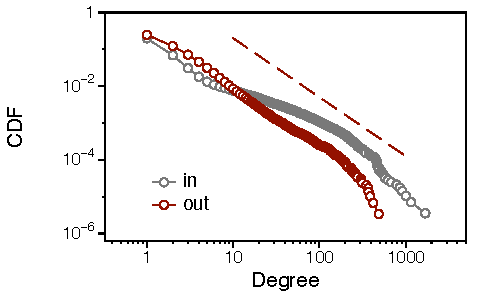
\includegraphics{HIT_Degree_CDF.pdf}
\caption{Degree distribution of the livestock trade network. The out-degree distribution (red circles) is well approximated by a power-law of the form $x^{-1.67}$ (red dashed line).
The in-degree distribution shows a bimodal behavior indicating the presence of large slaughterhouses (grey triangles).
Power law exponent was computed using a maximum likelihood estimator \citep{Clauset:2009}.
}
\label{fig:hit_deg_cdf}
\end{SCfigure}
%

\subsection{Components and ranges}
% all: 121223 nodes
% LWCC: 119858, 2nd: 8
% LSCC: 34693, 2nd: 16
Ignoring the edge direction, the network has a giant component containing almost 99~\% of the nodes. The second largest weakly connected component contains only 8 nodes.
The size of the largest and second largest strongly connected components are 28,6~\% (34,693 nodes) and  0.01~\% (16 nodes), respectively.
Sizes of the next smaller components decrease rapidly.
All in all the network percolates ignoring the direction of links.
Taking into account link directions, the giant component contains a considerable fraction of the network, but is far from the percolation threshold.

The giant strongly connected component has an interesting impact on the distribution of node ranges (and reachabilities) in the network.
Note that the range of a node defines the upper bound for any disease outbreak starting from this very node.
Following equation \eqref{eq:range_def}, we compute the ranges of all nodes and focus for the moment on the \emph{sequence} of these ranges. 
For most sequences of centralities in a network, we would find rather noisy signals.
These signals result in distributions such as the degree distribution in figure \ref{fig:hit_deg_cdf}.
In contrast to most other centrality measures, the range shows a strikingly different behavior.
The sequence of ranges for all nodes in the network is shown in figure \ref{fig:node_range}. 
%
\begin{figure}[htbp]
\begin{center}
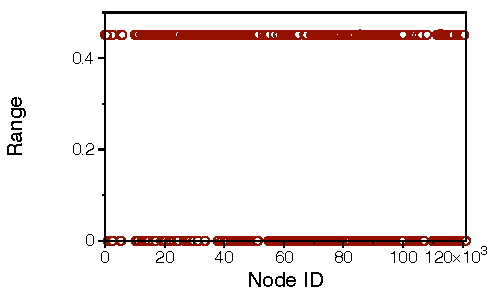
\includegraphics{Node_Range_PVM_100th.pdf}
\caption{Range sequence for all nodes in the livestock trade network.
The sequence shows a clear gap in the possible range values and a smaller second gap for the top ranged nodes.
Every 100th node with range greater than 0 is shown.
}
\label{fig:node_range}
\end{center}
\end{figure}
%
The striking feature here is the \emph{gap} in the distribution: no range in between $7\cdot 10^{-4}$ (87 nodes) and $0.45$ (54693 nodes) is present in the system.
%There is another, smaller gap for values between $0.33$ (29325 nodes) and $0.35$ (31033 nodes).
Consequently, a randomly chosen node can only belong to one of two classes, namely long ranged nodes and short ranged nodes.
A node of the latter class is barely suitable to cause a considerable disease outbreak at all.
Only a node of long range can act as a node for large scale disease outbreaks.
The sizes of the classes in figure \ref{fig:node_range} are as follows: 54,874 nodes belong to the short range and 66,349 nodes to the long range class, respectively.
%91 nodes of the latter are above the second range gap.

For a general network we define the range gap $\Gamma $ as the size of the largest interval, where the range distribution is identically zero \citep{Lentz:2012pre}.
The balance of the distribution around the gap is measured in terms of the variable
\[
b=\frac{N_l-N_s}{N},
\]
where $N=N_l+N_s$ is the number of nodes and $N_l$ and $N_s$ are the numbers of long and short ranged nodes, respectively.
Apparently $b=1$, if all nodes are long ranged and $b=-1$ for only short ranged nodes in the network.
Figure \ref{fig:ER_range_gaps} shows the range gap and balance for directed \ER networks of varying density.
The figure demonstrates, that the size of the range gap and the balance are inherently related to the percolation properties of the system (see section \ref{sec:er_model}).
A significant range gap in combination with equally sized range classes indicates that the system is in a critical state.
The author would like to stress the fact that the combination of range gap and balance is a more general indicator for the critical state than the average degree (see figure \ref{fig:ER_lcc_emergence}, section \ref{sec:er_model}).
This is because the range gap is not subject to any random model assumption.
For the dataset of figure \ref{fig:node_range} we get $\Gamma = 0.45$ and $b=0.095$ indicating that the system is only slightly above the critical point.
Note that for the undirected case, the range of every node is equivalent to the size of the component it belongs to.
Thus, ranges show a rather trivial behavior in the undirected case.
%
\begin{SCfigure}
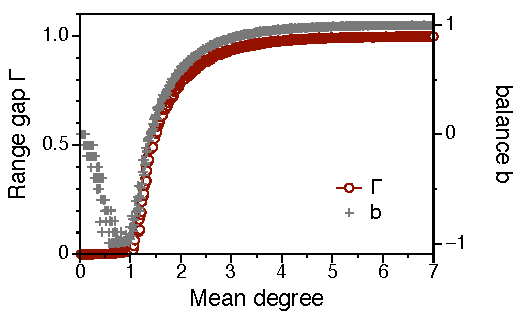
\includegraphics{ER_Range_gap.pdf}
\caption{Range gap $\Gamma $ and balance $b$ vs. mean degree for directed \ER graphs.
Each datapoint is a mean value of 1000 networks. Network size: 1000 nodes.
}
\label{fig:ER_range_gaps}
\end{SCfigure}

The explanation for the strong bi-modality of the range distribution is the existence of a giant strongly connected component (GSCC).
Figure \ref{fig:rangegap_principle} shows a schematic picture of a directed network.
Due to the giant component in the system, all nodes that belong to the GSCC can reach all other nodes in the component plus all nodes that the component is connected to.
%
\begin{figure}[htbp]
\begin{center}
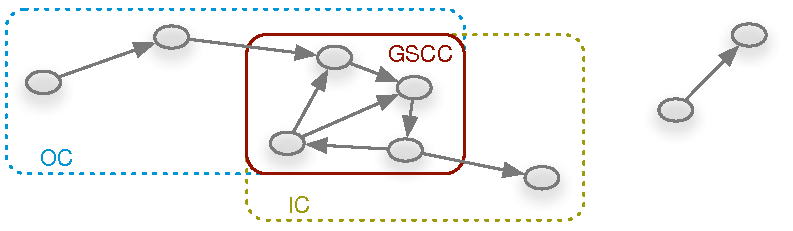
\includegraphics{RangeGap-principle.pdf}
\caption{Schematic structure of a directed network.
In the core region there is the giant strongly connected component (GSCC, red). All nodes reachable from the GSCC form the giant out-component (GOC, yellow) and the nodes with access to the GSCC define the giant in-component (GIC, blue).
The union of GSCC, GIC, GOC and all tendrils is the giant weakly connected component (GWCC) of the network.
Nodes that are not part of the GWCC belong to another component of the network (nodes on the upper right).
}
\label{fig:rangegap_principle}
\end{center}
\end{figure}
%
If there is a path from a node to the GSCC, but the node itself is not on this component, it belongs to the giant in-component (GIC) of the network. 
In analogy, nodes reachable from the GSCC that are themselves not part of the latter, belong to the giant out-component (GOC).
All remaining nodes not belonging to one of the components mentioned above are called tendrils, if they are weakly connected to the GSCC.
The nodes on the upper right (figure \ref{fig:rangegap_principle}) are not even weakly connected to the GSCC and thus belong to another component of the network.

As an explanation for figure \ref{fig:node_range}, the lower bound of the long range node class is formed by the nodes of the LSCC.
Every node that belongs to the long range node class is either on the LSCC or on the GIC.
The low range class is populated by nodes of the GOC, tendrils and nodes of other WCCs.

\subsection{Modules}
The network components analyzed above make a strict requirement to the connectivity between components.
A weaker requirement would be to allow for the existence of only a few edges between components.
Clusters of this type are called \emph{modules} or \emph{communities}.
The idea of finding modules in networks has been proposed in \citep{Newman06062006}.
In order to detect these structures, a cost function mapping every partition of the network onto a value between 0 and 1 has to be optimized.
\citeauthor{Newman06062006} proposed the modularity $Q$ as an appropriate cost function defined as
\[
Q=\text{(number of edges between communities)}-\text{(expected number of those edges)}
\]
or more formally \citep{Fortunanto2010,Newman06062006}
\begin{equation}\label{eq:modularity}
Q=\frac{1}{2m} \sum _{ij}\left( \mat{A}_{ij}-\frac{k_i k_j}{2m} \right) \delta (c_i,c_j).
\end{equation}
This equation gives the modularity for a network with adjacency matrix $\mat{A}$ and $m$ edges and $k_i$ denotes the degree of the $i$-th node.
%
\begin{SCfigure}
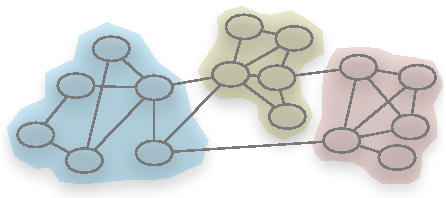
\includegraphics{Module_Prinzip-06diss.pdf}
\caption{The nodes of modular networks are partitioned into modules of high edge density and edges between modules are rare.}
\label{fig:modular_principle}
\end{SCfigure}

%
The partition of the network is given in the Kronecker delta $\delta (c_i,c_j)$, which is 1, if nodes $i$ and $j$ are in the same community and otherwise 0.
Hence, modularity measures the goodness of a particular partition of the network.
$Q\sim 0$ implies that a given partition of a network does not give a significant modular structure.
Its maximum value is $Q=1$ provided that a network has a strong modular partition \emph{and} the latter is known for the computation of $Q$.
Finding best possible partition that maximizes modularity has been shown to be NP-complete \citep{brandes2007}.
However, several approximate methods -- such as simulated annealing \citep{guimera_mod_SA} and greedy algorithms \citep{Clauset_greedy,Newman:fast_algo} -- to maximize modularity have been proposed.
In order to detect community structure in the pig trade network, we analyze the system using the method of \citeauthor{Newman:fast_algo}.
The results presented in this section are published in \citep{Lentz:2011}.
%\footnote{We show results computed for the pig trade data set within observation period 01 june 2006 and 31 december 2008, as in \citep{Lentz:2011}.
%Results remain qualitatively the same for the dataset 01 january 2009 -- march 2010.

Note that we focus on the partition of only the undirected network.
Although the concept of modularity can be generalized to the directed case in a straightforward manner using the definition \citep{Leicht:2008p5144}
\begin{equation}\label{eq:directed_modularity}
Q=\frac{1}{m} \sum _{ij}\left( \mat{A}_{ij}-\frac{k_i ^- k_j ^+}{m} \right) \delta (c_i,c_j),
\end{equation}
there is still ongoing discussion about a systematic bias in this approach \citep{kim2010}.
\citeauthor{kim2010} point out that a straightforward generalization of modularity can not resolve nodes of different in and out degree. 
Hence, nodes of high total degree tend to form communities with their neighborhood regardless of how the links in the neighborhood are directed.

In order to find a partitioning maximizing the modularity function \eqref{eq:modularity}, we use the greedy method proposed in \citep{Clauset_greedy}.
The algorithm was applied to the largest weakly connected component of the network, i.e. $119,858$ nodes.
It finds a partition where 96~\% of all nodes and 98~\% of all edges are assigned to 9 major clusters.
The modularity value for this partition is $Q=0.717$.
After we computation of a suitable network partition, we add the geographical positions of the nodes as further meta information.
The resulting map is shown in figure \ref{fig:D9}.
It should be noted that the community partition was done without spatial information in the first place.
Thus, the figure demonstrates that in this case two nodes of the same community are likely to be geographic neighbors as well.
An explanation for this correlation could be cultural affinity or simply economic reasons, since transport costs scale with geographical distance.

\begin{figure}[htb]
\begin{center}
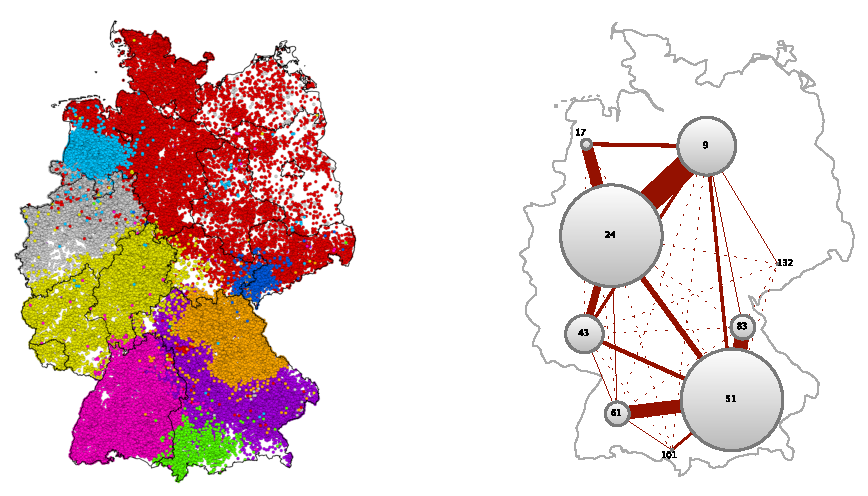
\includegraphics{D9.pdf}
\caption{Geographical embedding of the communities found for the pig trade network (left).
The nine largest (by number of nodes) communities are shown.
The number of edges between the communities and within the communities is shown on the right.
From \citet{Lentz:2011}.
}
\label{fig:D9}
\end{center}
\end{figure}

The right panel of figure \ref{fig:D9} shows the nine largest communities condensed into single nodes, where the size of each node represents the number of edges in the community.
Node numbers are arbitrary IDs given by the used algorithm.
Links between communities are weighted ranging from 6 (dashed lines) to 7251 (massive edge between 24 and 9).
The positions of the nodes approximate the center of mass of the corresponding community on the left panel.

Module detection is a reasonable tool for capturing the large scale structure of networks.
In fact, is has been shown that there is a resolution limit for community detection and the minimum size of the communities depends on the size of the network \citep{SantoFortunato01022007}.
In general, meta information such as the geographical embedding of the network, is needed to gain knowledge about the function of a network out of its structure.

A particular partitioning of a network, however, is not guaranteed to give unambiguous information about the network.
On the contrary, equation \eqref{eq:modularity} is a mapping from a high dimensional partition space to a scalar.
The number of elements in the partition space is given by the \emph{bell number}.
This implies that the number of partitions of a network with 10 nodes is $\sim 10^5$ and it is already $\sim 10^{47}$ for 50 nodes!
Adjacent partitions in the partition space can have huge differences in $Q$ and it is not guaranteed that approximative algorithms are capable to find the global optimum.
Furthermore, a huge number of different partitions can possess the same modularity $Q$.

Although a particular partition should in general be interpreted with caution, we can state that \emph{at least one} partition of a certain value of $Q$ is intrinsic in the system.
I.e. the system is somehow modular, even if the best possible partition might be unknown.
We consider this line of thought in the next section, where we analyze artificial networks with distinctive structural features in order to gain insight into their impact on epidemic processes.

\section{Range \& modules: Spreading potential}\label{sec:PRE}
In this section, we investigate the impact of directionality and modularity of networks on epidemic processes.
Therefore, we use random network models that mimic the desired properties.
To begin with, we derive a system of equations that models an epidemic process as it would take place on the pig trade network of section \ref{sec:network_analysis}.
For this reason, we consider the agricultural holdings as meta-populations and the time scales between trade and infection are separated using a pacing of trade.
All results presented in this section are published in \citep{Lentz:2012pre}.

\subsection{Epidemic model}
In this section, we derive an infection model for agricultural holdings that are considered as meta populations, each holding containing a certain number of animals. 
The coupling between the holdings is given by trade, which appears as transportation of livestock animals (see figure \ref{fig:metapop_scheme}).
The union of all trade couplings is given by a trade network with adjacency matrix $\mat{A}$. 
Since transportation/trade in this sense is a non symmetric process, we focus on \emph{directed networks} in particular.

In each node of the network, a susceptible-infected-recovered (SIR) reaction takes place.
Following section \ref{sec:sir_model}, the infection model for each node $\mu $ in such a system reads
\begin{align}\label{eq:local_sir_only}
\partial _t s_\mu &= -\alpha s_\mu \frac{i_\mu}{n_\mu} \notag \\
\partial _t i_\mu &=  \alpha s_\mu \frac{i_\mu}{n_\mu} - \gamma i_\mu \notag \\
\partial _t r_\mu &= \gamma i_\mu ,
\end{align}
where $n_\mu =s_\mu + i_\mu + r_\mu $ is the total population of node $\mu $ and we use the force of infection $i_\mu / n_\mu $ as suggested in equation \eqref{eq:force_of_infection}.
The \emph{infection status} of node $\mu $ is given by the triple $(s_\mu , i_\mu , r_\mu )$.
Now we add the interactions between the meta populations by introducing a network with adjacency matrix elements $a_{\mu \nu }$.

The total \emph{outflow} from node $\mu $ is given by its degree $\sum _\nu a_{\mu \nu }$ and divides into
\[
f_\mu ^- =  \frac{s_\mu }{n_\mu} \sum _\nu a_{\mu \nu } + \frac{i_\mu }{n_\mu} \sum _\nu a_{\mu \nu }+ \frac{r_\mu }{n_\mu} \sum _\nu a_{\mu \nu }
\]
according to the infection status of the node.
The \emph{inflow} of each node depends on the infection status of its predecessors in the network, i.e.
\[
f_\mu ^+ =\sum _\nu a^T _{\mu \nu }\frac{s_\nu }{n_\nu } + \sum _\nu a^T _{\mu \nu }\frac{i_\nu }{n_\nu } + \sum _\nu a^T _{\mu \nu }\frac{r_\nu }{n_\nu },
\]
where $\sum _\nu a^T _{\mu \nu }=\sum _\nu a _{\nu \mu }$ is the in degree of node $\mu $.
We add the respective contributions of inflow and outflow to equations \eqref{eq:local_sir_only} and get
%
\begin{align}
\partial _t s_\mu &= -\alpha s_\mu \frac{i_\mu}{n_\mu} + \sum _\nu a^T _{\mu \nu} \frac{s_\nu }{n_\nu } - \frac{s_\mu }{n_\mu }  \sum _\nu a_{\mu \nu} \notag \\
\partial _t i_\mu &=  \alpha s_\mu \frac{i_\mu}{n_\mu} + \sum _\nu a^T _{\mu \nu} \frac{i_\nu }{n_\nu  } - \frac{i_\mu }{n_\mu  }  \sum _\nu a_{\mu \nu} -\gamma i_\mu \notag \\
\partial _t r_\mu &= \sum _\nu a^T _{\mu \nu} \frac{r_\nu }{n_\nu } - \frac{r_\mu }{n_\mu }  \sum _\nu a_{\mu \nu} +\gamma i_\mu .
\label{eq:sir_indices_pre} 
\end{align}
%
Regarding this equation system, we have to address the impact of directionality, i.e. the non-symmetry of the adjacency matrix.
Considering the coupling term in equations \eqref{eq:sir_indices_pre}, we have to make sure that the population of each node remains constant, i.e. $f_\mu ^- = f_\mu ^+$.
Using that $\frac{s_\nu}{n_\nu} +\frac{i_\nu}{n_\nu} +\frac{r_\nu}{n_\nu} =1$ this is equivalent to the condition
\[
\sum _\nu (a_{\nu \mu }-a_{\mu \nu})=0.
\]
In undirected networks, this condition is always satisfied.
In directed networks, however, the condition implies that each node in the network has the same in and out degree, respectively.
This does not hold in the general case, so that the total flow of node $\mu $ is
\[
\sum _\nu (a_{\nu \mu }-a_{\mu \nu})= f_\mu ^+ -f_\mu ^- \equiv f_\mu \neq 0 ,
\]
i.e. the difference between in-degree and out-degree.
This difference is distributed over the infection status of the respective node so that
\[
f_\mu =\frac{s_\mu }{n_\mu }f_\mu ^s +\frac{i_\mu }{n_\mu }f_\mu ^i +\frac{r_\mu }{n_\mu }f_\mu ^r .
\]
It follows that in the case of a directed network, we have to add a birth/death process in each node to keep the total population constant.
Hence, the infection model becomes
%
\begin{align}
\partial _t s_\mu &= -\alpha s_\mu \frac{i_\mu}{n_\mu} + \sum _\nu a^T _{\mu \nu} \frac{s_\nu }{n_\nu } - \frac{s_\mu }{n_\mu }  \sum _\nu a_{\mu \nu} -\frac{s_\mu }{n_\mu } f^s _\mu \notag \\
\partial _t i_\mu &=  \alpha s_\mu \frac{i_\mu}{n_\mu} + \sum _\nu a^T _{\mu \nu} \frac{i_\nu }{n_\nu  } - \frac{i_\mu }{n_\mu  }  \sum _\nu a_{\mu \nu} -\gamma i_\mu -\frac{i_\mu }{n_\mu } f^i _\mu \notag \\
\partial _t r_\mu &= \sum _\nu a^T _{\mu \nu} \frac{r_\nu }{n_\nu } - \frac{r_\mu }{n_\mu }  \sum _\nu a_{\mu \nu} +\gamma i_\mu -\frac{r_\mu }{n_\mu } f^r _\mu .
\label{eq:sir_indices_with_flow_correction} 
\end{align}
%
In analogy to section \ref{sec:network_matrices}, we define the Laplace Matrix $\mat{L}$ with elements
\begin{equation}\label{eq:sir_laplace}
l_{\mu \nu} = a^T _{\mu \nu } - \delta _{\mu \nu }\sum _\sigma a_{\mu \sigma } .
\end{equation}
Using vector notation, the status of the whole network is given by the respective vectors $\mat{S}$, $\mat{I}$ and $\mat{R}$.
Lowercase letters refer to normalized variables, i. e. the elements of $\mat{s}$ are $s_\mu / n_\mu $.
the system \eqref{eq:sir_indices_with_flow_correction} now reads
\begin{align}\label{eq:sir_no_pacing}
\partial _t \mat{S} &=\mat{L}\mat{s}- \mathrm{diag} (\mat{s}\mat{F}_s)-\alpha \; \mathrm{diag}(\mat{S}\mat{i}) \nonumber \\
\partial _t \mat{I} &=\mat{L}\mat{i}- \mathrm{diag} (\mat{s}\mat{F}_i)-\alpha \; \mathrm{diag}(\mat{S}\mat{i}) -\gamma \mat{I} \nonumber \\
\partial _t \mat{S} &=\mat{L}\mat{r}- \mathrm{diag} (\mat{r}\mat{F}_r) +\gamma \mat{I} .
\end{align}
This system models an SIR-type epidemic on a meta population which is connected by a network structure given by the Laplacian $\mat{L}$.
In \eqref{eq:sir_no_pacing}, $\mathrm{diag} (\mat{x} \mat{y})$ denotes the main diagonal of the outer product of vectors $\mat{x}$ and $\mat{y}$.

Still, the infection time scale is the same as the trade time scale in \eqref{eq:sir_no_pacing}.
In order to separate these time scales, we modify the Laplacian \eqref{eq:sir_laplace} and define a \emph{paced Laplacian}
\begin{equation}\label{eq:new_laplacian}
\mathcal{L}(\tau )=\mat{L} \sum _{n=0} ^\infty  \delta (t-n\tau )
\end{equation}
with pacing frequency $\tau $.
Thus, we obtain the requested model replacing the Laplacian in \eqref{eq:sir_no_pacing} by its paced counterpart.
Finally , we use the following outbreak model:
%
\begin{align}\label{eq:sir_with_pacing}
\partial _t \mat{S} &=\mathcal{L}(\tau )\mat{s}- \mathrm{diag} (\mat{s}\mat{F}_s)-\alpha \; \mathrm{diag}(\mat{S}\mat{i}) \nonumber \\
\partial _t \mat{I} &=\mathcal{L}(\tau )\mat{i}- \mathrm{diag} (\mat{s}\mat{F}_i)-\alpha \; \mathrm{diag}(\mat{S}\mat{i}) -\gamma \mat{I} \nonumber \\
\partial _t \mat{S} &=\mathcal{L}(\tau )\mat{r}- \mathrm{diag} (\mat{r}\mat{F}_r) +\gamma \mat{I} .
\end{align}
%
In order to analyze the impact of characteristic topological features -- in particular modularity and directionality -- on disease dynamics, we solve equations \eqref{eq:sir_with_pacing} numerically for different computer-generated networks with the desired properties.

\subsection{Computer-generated networks}\label{sec:computer-gen-networks}
In this section we describe how networks with varying directionality and modularity can be generated on a computer.
Although generating a sequence of graphs with a certain directionality is straightforward, we have to discuss how to quantify this property.
Before we generate networks of a desired modularity, we address restrictions in the maximum value of $Q$.

\paragraph{Networks of varying directionality\color{Cayenne}{.}}
The directionality of a given network is related to its fraction of bidirectional links.
In principle, the strength of direction could be measured this way.
It has been shown, however, that this measure would yield finite values even for purely random networks \citep{Garlaschelli2004}.
Therefore, \citeauthor{Garlaschelli2004} introduced the measure of \emph{link reciprocity} $\rho $ of a given network with $N$ nodes and adjacency matrix $\mat{A}$ as
\begin{equation}\label{eq:link_reciprocity}
\rho =\frac{\sum _{i\neq j} (a_{ij}-\bar{a})(a^T _{ij}-\bar{a})}{\sum _{i\neq j} (a_{ij}-\bar{a})^2}.
\end{equation}
The edge density is denoted as $\bar{a}=\sum _{ij} a_{ij}/(N(N-1))$.
In fact, equation \eqref{eq:link_reciprocity} is the correlation between an adjacency matrix and its transposed.
Reciprocity $\rho =1$ for undirected networks, whereas $\rho \approx 0 $ for directed random graphs.
In the latter case the fraction of bidirectional links would take finite values, since some bidirectional links are taken by chance.

To investigate the impact of directionality on disease dynamics, we generate random networks with different values of $\rho $ and solve the system \eqref{eq:sir_with_pacing} on these topologies.
The networks are generated as follows:
1. generate an undirected \ER network, 2. replace all edges by bidirectional directed edge pairs and 3. remove one edge of the bidirectional edge pair with probability $q$.
Consequently, the probability that an edge pair is connected by an undirected (bidirectional) edge is $p_\mathrm{rev} = 1-q$.
The link reciprocity of the generated network can directly be computed using equation \eqref{eq:link_reciprocity}.
We have to point out that this analysis focuses on \ER networks.
Other network types are possible as well, but would add more complexity to the analysis.  

\paragraph{Modular networks\color{Cayenne}{.}}
Following \citeauthor{Newman:2004}, a modular network can be realized as a union of independent subgraphs, that are afterwards sparsely connected \citep{Newman:2004}.
In this work, we use random networks with fixed node number $N$ and edge probability $p$ as subgraphs.
The connection of subgraphs is achieved by by placing edges between them with probability $p_\mathrm{out}$.
Varying $p_\mathrm{out}$ allows for an adjustment of the modularity $Q$, which is computed using equation \eqref{eq:directed_modularity}.

It should be noted that a sufficient number of subgraphs is necessary to obtain large values of $Q$.
We found an analytic approximation for the maximum possible modularity by maximizing equation \eqref{eq:modularity} (or \eqref{eq:directed_modularity}, respectively) for different module numbers. 
For a network of $n$ modules the maximum modularity is
\begin{equation}\label{eq:Q_max}
Q_\mathrm{max}=1-\frac{1}{n}.
\end{equation}
Derivation sketch: given a modular network with adjacency matrix $\mat{A}$, there is always a relabeling of indices $\mat{P}$ so that $\mat{A}'=\mat{P}\mat{A}\mat{P}^{-1}$ is block diagonal.
The maximum modularity can be derived from the blocks of $\mat{A}'$, since the graphs of $\mat{A}'$ and $\mat{A}$ are isomorphic.
A full derivation of \eqref{eq:Q_max} is given in Appendix \ref{sec:maximum_modularity_subgraphs}.

\subsection{Impact of directionality}\label{sec:impact_directionality}
We solve the system \eqref{eq:sir_with_pacing} on a sequence of networks as generated according to the previous section.
For the rest of this work, we keep the following parameters constant:
The infection parameters are $\alpha =3$, $\gamma = 1$, $\tau =21$.
The initial infection status of all nodes are $(s_\mu (0),i_\mu (0),r_\mu (0))=(300,0,0)$.
As initial conditions, we choose the node with longest range to avoid trivial solutions and its initial state is $(299,1,0)$.
Figure \ref{fig:typical_trajectory} shows a typical solution of the system on a random network.

\begin{SCfigure}
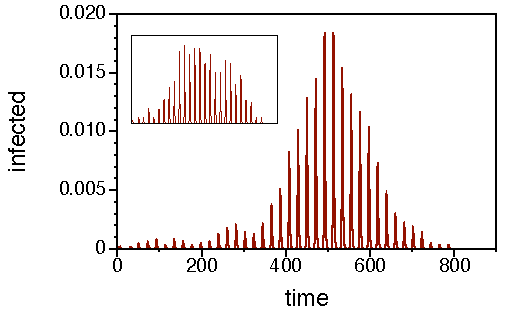
\includegraphics{Typical_Trajectory.pdf}
\caption{Typical infection curve $\sum _\nu i_\nu (t)$ of a solution of equation \eqref{eq:sir_with_pacing}.
The ratio of $1/\tau $ and $\gamma $ results in a comb shape of the infection curve.
Inset shows the more noisy infection curve of a critical network.
Networks: \ER network with 2000 nodes, $p=0.05$, $p_\mathrm{rev}=0.5$ (inset: $p=0.001$, $p_\mathrm{rev}=0.01$).
From \citep{Lentz:2012pre}.
}
\label{fig:typical_trajectory}
\end{SCfigure}

Although the choice of parameters seems a bit arbitrary in the first place, the qualitative behavior of the system depends only weakly on the exact parameter values \citep{Lentz:2012pre}.
We have seen in section \ref{sec:sir_model} that the outbreak condition \eqref{eq:r0} determines whether an outbreak occurs at all.
Above threshold, SIR-type outbreaks show quasi similar behavior.
That is why the fraction $\alpha / \gamma $ in equations \eqref{eq:sir_with_pacing} is of minor importance as long as $\alpha / \gamma >1$.
In addition to that, the characteristic time scale of an SIR infection is given by $1/\gamma $ (see equation \eqref{eq:sir_characteristic_time_scale_gamma}).
If the pacing of the network coupling $\tau $ is too slow, a local infection dies out before it can be moved to the next node.
Therefore, we choose $\tau $ and $\gamma $ so that an infection can spread along the network.
An analysis of the outbreak dynamics in the $(\tau \gamma)$ parameter space is given in \citep{Lentz:2012pre}.

After integrating the system \eqref{eq:sir_with_pacing} on computer generated networks, we compute the final size of epidemic (see section \ref{sec:sir_model})
\[
R_\infty = \lim _{t\rightarrow \infty } \sum _\nu r_\nu (t),
\]
which is normalized by the population size $P$ to yield the outbreak size
\begin{equation}\label{eq:pre_outbreak_size}
r_\infty =\frac{R_\infty}{P}.
\end{equation}
Figure \ref{fig:outbreaksize_vs_rec_ER} shows the outbreak size for \ER networks with different values of link reciprocity.
The plot shows networks of different densities determined by the edge occupation probability $p$.
Note that $p$ corresponds to the edge density before edge removal as described in section \ref{sec:computer-gen-networks}.
Hence, the edge density is further reduced for smaller values of $\rho $.
%
\begin{figure}[htb]
\begin{center}
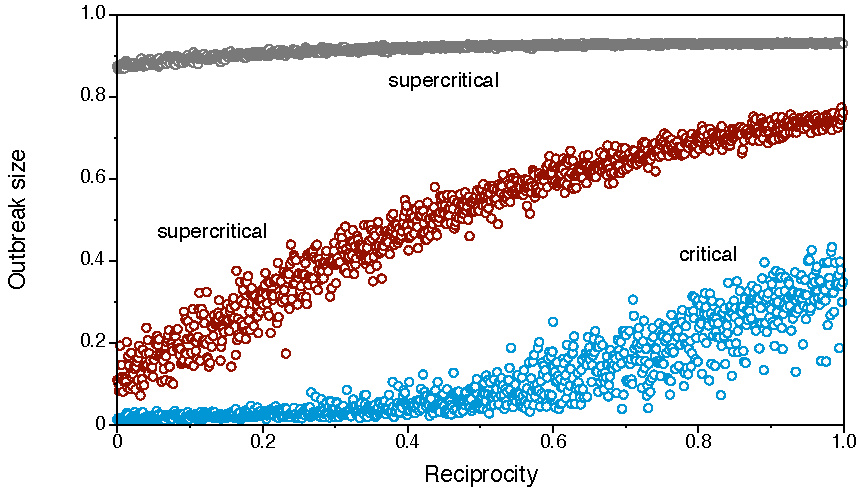
\includegraphics{Outbreaksize_vs_rec_ER.pdf}
\caption{Effect of directionality for an SIR outbreak on a random network.
Each point corresponds to one outbreak simulation on one network.
All networks have 2000 nodes.
Initial network densities: grey: $p=0.003$, red: $p=0.001$, blue: $p = 0.000625$.
From \citep{Lentz:2012pre}.
}
\label{fig:outbreaksize_vs_rec_ER}
\end{center}
\end{figure}

Grey points in figure \ref{fig:outbreaksize_vs_rec_ER} represent outbreaks in rather dense ($p=0.003$) networks.
This density is significantly larger than the percolation threshold of the network, which is $p_c=0.0005$.
Thus, the networks are clearly supercritical.
The figure demonstrates that the outbreak size is almost constant for all values of $\rho $, indicating that the high link density of the network is not affected by a removal of some bidirectional links.
The red points also represent outbreaks on supercritical networks, but the densities of the networks are only slightly above the critical point.
As a consequence, the outbreak size is more sensitive to changes of reciprocity.
The outbreak size range from $0.1$ to $0.8$ in this case.
The density of the blue outbreaks correspond to networks with initial density $p=0.000625$.
Consequently, the density is approximately $0.0005=p_c$ for $\rho =0.5 $.
This implies, that the network undergoes a phase transition for $\rho =0.5$.
As shown in the figure, the outbreak size depends on the link reciprocity only in the supercritical regime.

The findings of figure \ref{fig:outbreaksize_vs_rec_ER} demonstrate, that the structure of the underlying network affects the outbreak size. In particular, critical networks show a strong sensitivity to changes in directionality.
Nevertheless, it can be shown that the effect behind the results in figure \ref{fig:outbreaksize_vs_rec_ER} is not due to mixing of the population, but can in fact be explained by purely topological arguments \citep{Lentz:2012pre}.
This is shown by comparing the range of the initially infected node with the actual size of the disease outbreak.
A deviation between the two would indicate that back-mixing of recovered into the population is responsible for a decrease in outbreak size, since recovered do not contribute to the infection process, but can act as infection firewalls.

\subsection{Impact of modularity}\label{sec:impact_of_modularity}
Before we study the impact of modularity, we define the \emph{time of outbreak peak} in order to quantify the time period of the main epidemic.
The peak time of the epidemic is defined as the time, that divides the infection curve into two equal areas, i.e. the ``median'' of the infection curve.
Since this corresponds to the time, where half of the final infection size is reached.
It follows from the SIR model \eqref{eq:sir_model} that the time of infection peak can also be computed using
\begin{equation}\label{eq:pre_time_of_infection_peak}
t: i(t)= R_\infty /2 .
\end{equation}
Using the term ``median'', the number of recovered is -- up to a constant -- the ``cumulative distribution'' of the infection curve, i.e $dR/dt=\gamma I$.

As in the previous section, we compute the outbreak sizes and the infection peak times for networks of different modularity generated according to section \ref{sec:computer-gen-networks}.
For each outbreak, we compute the outbreak size $r_\infty $ following \eqref{eq:pre_outbreak_size} and the time of infection peak as defined in \eqref{eq:pre_time_of_infection_peak}.
The results are shown in figure \ref{fig:time_rinfty_vs_mod}.
%
\begin{figure}[htb]
\begin{center}
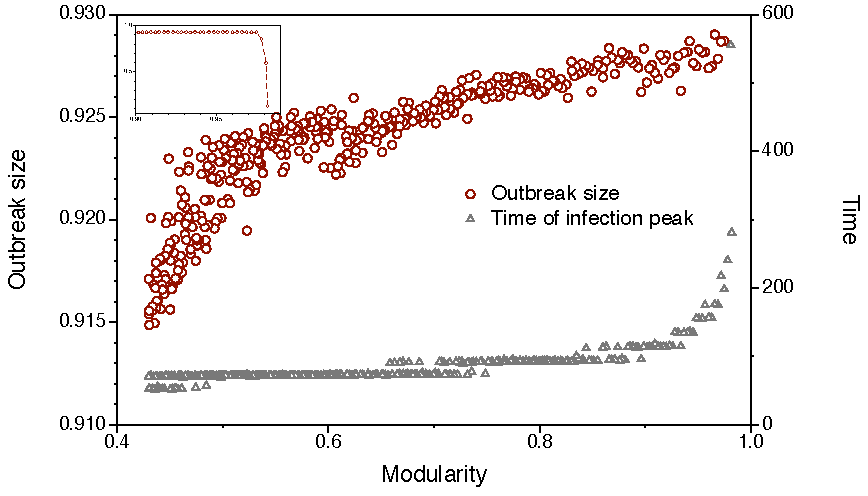
\includegraphics{Outbreaksieandtime_vs_Q}
\caption{Impact of modularity $Q$ on the outbreak size $r_\infty $. The outbreak size (red circles) is affected by an increase of modularity, although the effect is rather weak.
The inset shows the disintegration of the network resulting in a drop of the outbreak size for very large values of $Q$.
Grey triangles demonstrate that increasing modularity can cause significant delays of the infection peak.}
\label{fig:time_rinfty_vs_mod}
\end{center}
\end{figure}

As the figure demonstrates, the size of infection increases with modularity (red circles).
This can be explained by the distribution of recovered and infected:
In the early phase the epidemic is localized in the initial module, while it is unlikely that other modules become infected in the first place.
Modules have a high link density by definition so that an infection is likely to infect large parts of the initial module in the early phase.
In the moment when a path is accessible to another module, the new module is likely to comprise of a large number of susceptible population.
Therefore, the recovered subpopulation cannot act as a firewall against infection spread.

It should be noted that the effect is marginal over a wide range of modularity.
The inset shows that a very high modularity causes a significant drop of the outbreak size, since the network disintegrates into disconnected components in this limit.
In contrast to the effect discussed above, the drop of outbreak size in the limit $Q\rightarrow 1$ is a purely topological one \citep{Lentz:2012pre}.
This can be shown with the same arguments as in section \ref{sec:impact_directionality}.

In addition to that, figure \ref{fig:time_rinfty_vs_mod} shows the time of infection peak for different modularities (grey triangles).
For small and intermediate values of $Q$, we observe a slight delay of the outbreak peak.
The quantified behavior of the plot stems from the pacing $\tau $ of the network.
The main finding of the figure is that large values of modularity cause a significant delay of the outbreak peak.
This knowledge could be useful for the implementation of counter measures, such as vaccination strategies.
Consequently, there is more time to react in high modular networks.


\subsection{Impact of reciprocity in modular networks}
In this section, we focus on modular networks with varying link reciprocity, i.e. we combine the properties studied in sections \ref{sec:impact_directionality} and \ref{sec:impact_of_modularity}.
We generate a number of modular networks and change their link reciprocity afterwards.
Solving the infection model \eqref{eq:sir_model} on these topologies gives outbreak sizes for different reciprocities.
The results are shown in figure \ref{fig:outbreak_vs_rec_modular}.
%
\begin{figure}[htb]
\begin{center}
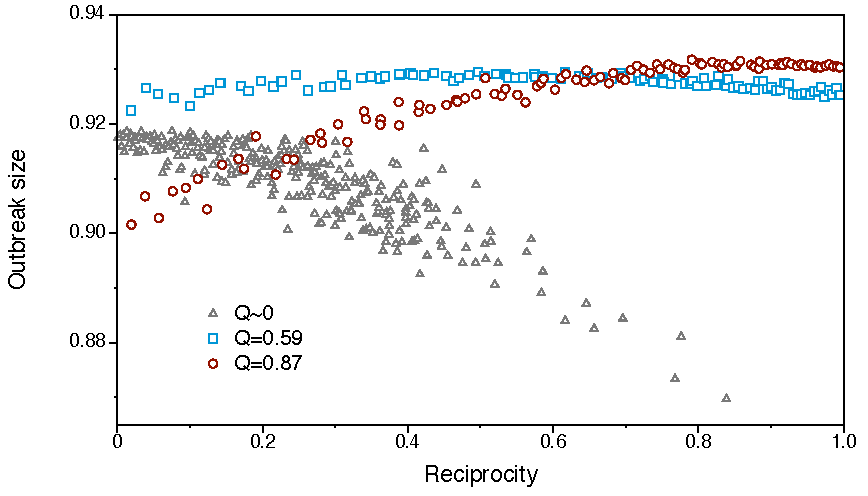
\includegraphics{Outbreaksize_vs_rec_modular.pdf}
\caption{Outbreak size vs. link reciprocity for modular networks.
Changing reciprocity in intermediate modular networks (blue squares) does not affect the outbreak size significantly.
Highly modular networks (red circles) act as isolated modules and show a behavior similar to that of figure \ref{fig:outbreaksize_vs_rec_ER}.
The correlation between outbreak size and reciprocity is reversed for very low modular networks (grey triangles)}
\label{fig:outbreak_vs_rec_modular}
\end{center}
\end{figure}

The red circles in figure \ref{fig:outbreak_vs_rec_modular} represent networks with $Q=0.87$, i.e. highly modular networks.
The outbreak size shows a behavior comparable to that of the supercritical \ER graphs in figure \ref{fig:outbreaksize_vs_rec_ER}.
This provides evidence for the hypothesis that the modules of highly modular networks act as isolated subgraphs.
For networks of intermediate modularity ($Q=0.59$, blue squares), there is almost no correlation between outbreak size and link reciprocity.

Interestingly, the correlation between outbreak size and link reciprocity becomes even negative for networks of very low modularity ($Q\sim 0$, grey triangles).
Grey triangles should not be confused with random networks.
In fact, they are generated as modular networks, but with very high inter-module edge probabilities $p_\mathrm{out}$, i.e. they possess an internal structure, but this structure is not resolved by the modularity any more.
This can can be seen as a limit $Q\searrow 0$.
A possible explanation for the counter-intuitive behavior of low modular networks is that there is a high probability that an infected subpopulation $M$ is highly connected to the module $M_0$ where the infection originated from.
As a matter of fact, the module $M_0$ is in an ``older'' infection state, i.e. it is dominated by recovered population.
Consequently, the effective number of susceptible population is decreased for this infection path and the spreading range is reduced.

\paragraph{Conclusion of the section\color{Cayenne}{.}}
The German pig trade network was analyzed in terms of static network measures.
Our main observations are the following:
First off, the system possesses a heavy-tailed degree distribution (figure \ref{fig:hit_deg_cdf}) indicating that the system is heterogenous and be vulnerable to epidemics (see section \ref{sec:epi_networks}).
Second, the network components and the distribution of ranges result in a node classification into either long range or short range nodes.
Any ranking of nodes according to their potential of disease spread is reduced to the class membership of the nodes in this context.
In addition to that, the balance $b$ of the range distribution provides evidence that the system considered here is in a critical state ($b=0.069$, see also figure \ref{fig:ER_range_gaps}).
The directionality of the network is inherently related to the gap seen in the range distribution.
An undirected network would not show a two class distribution.
Third, the network under consideration can be partitioned into modules, i.e. relatively densely connected subgraphs.
By adding meta-information (in this case geographical information) to the network partition, we found a reasonable partition into compact geographical regions (see figure \ref{fig:D9}).
The large scale trade structure of the system can be revealed this way.

Finally, the observations above raise two questions for the context of epidemics on networks:
1. how do link directions affect an epidemic outbreak? and
2. given a network is somehow modular, does this have any impact on disease dynamics?
In order to answer these questions, we generated random networks that allow for  a variation of the desired properties -- directionality and modularity -- and solved an infection model tailor made for a livestock trade network on these topologies.

Our main findings are: 1. Modularity can cause a significant delay of an outbreak, 2. stronger link directionality generally reduces the outbreak size, but in special topologies the effect can also be reversed.



%
%\bibliographystyle{apalike}
%\bibliography{/Users/lentz/Documents/GitHub_locals/Thesis/bibliography.bib}
%\end{document}

